\section{Introduction}

Autonomous navigation in unknown or semi-structured environments is one of the fundamental problems in mobile robotics. Even relatively simple maze environments introduce multiple practical challenges, including noisy sensor measurements, imperfect localization, unstable control loops, and mechanical inaccuracies of the robot platform.

The goal of this project was to design and implement a fully autonomous robot capable of navigating through a maze environment while reacting to visual navigation hints and maintaining stable movement inside corridors. The project was developed as part of the BPC-PRP course and combines multiple robotics disciplines into a single integrated system.

The implemented robot uses several sensing modalities simultaneously:\newline
- LiDAR for corridor detection and distance estimation\newline
- IMU for orientation tracking and turning stabilization\newline
- Wheel encoders for odometry feedback\newline
- Reflective line sensors for line following\newline
- Camera for ArUco marker recognition

The complete software solution was implemented using ROS2 and modular C++ nodes. The modular architecture allowed independent testing of individual subsystems and simplified debugging during development.

\begin{figure}[h]
    \centering
    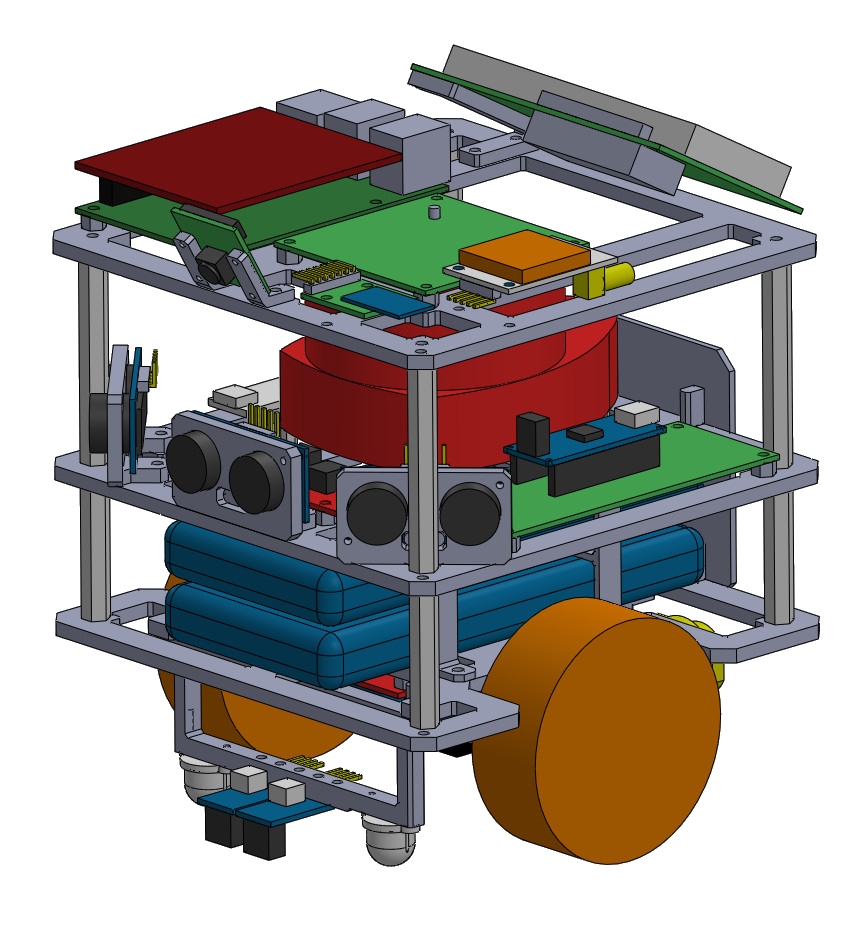
\includegraphics[width=0.45\textwidth]{images/render.png}
    \caption{Implemented autonomous robot platform [3]}
    \label{fig:robot}
\end{figure}

